\documentclass[12pt,journal,compsoc]{IEEEtran}

\usepackage{amsmath}
\usepackage{graphicx}
\usepackage{float}
\usepackage[hidelinks]{hyperref}
\hypersetup{% this is so dank I've been trying to do this FOREVER
colorlinks=true,% all links are colored and not outlined
linkcolor=black,% hyperlink (PDF internal links like in toc) colors will be black
urlcolor=blue,
citecolor=black
}

\begin{document}
\sloppy

\title{Telemetry, Control Systems, and Sensors on an Autonomous Aircraft}
\author{Maxwell~Bradley, Kodiak~North, and Zane~Bradley}

\date{\today} % leaving the brackets empty omits the date
% To input the current date, you can type: \date{\today}

% The paper headers
\markboth{Autonomous Aerial Wildfire Detection}{Bradley, M; North, K; Bradley, Z}

\IEEEcompsoctitleabstractindextext{%
\begin{abstract}
This paper describes the subsystems onboard an autonomous aircraft that detects wildfires. The first subsystem is the 
data transfer system, between the aircraft and the ground. The second is the control system, which navigates the plane
between predefined way points, and keeps it on course in the event of wind or thermals. The third system is the 
fire detection system, which scans incoming images, determines if there is a fire present, and communicates with the 
data transfer system in the event of a fire.
\end{abstract}

\begin{IEEEkeywords}
Aircraft, Airplane, RC Airplane, UAV, Autonomous, Wildfire, Wildfire Detection, Search and Rescue
\end{IEEEkeywords}}

\maketitle

\tableofcontents 
\newpage
\section{Project Introduction}

\IEEEPARstart{F}{orever} Flight is a persistent aerial monitoring system to detect wildfires in fire-prone areas. It will consist of a plane with a mounted IR camera to detect fires below and a flight controller capable of autopilot, guidable with GPS waypoints sent from a laptop computer on the ground. This project was named `Forever Flight' for its goal of never having to recharge its batteries, staying aloft and performing fire detection while the sun is up, charging back up from solar energy and our power regenerative mechanisms. 

This project was inspired by the recent California wildfires like the Camp Fire, a 2018 fire in Northern California that caused \$16.5 billion in damage and claimed 86 lives [1]. The reason that these fires were so deadly is because there was no early warning system that detected the fire before it started ripping through towns like Paradise, California. The team hopes that Forever Flight will prevent fires like this.

% MAX B
\section{Data Transfer}
\subsection{Introduction}
There is a large amount of information coming out of the aircraft at any time, transferred over telemetry. This transfer contains a huge amount of different kinds of data, such as fire detection stats, fire detection processing, GPS coordinates, and more. Getting this kind of information out of the plane can be challenging because of the flight controller's running overhead and varying transmission protocol versions. I will focus this section of the paper on the transfer of data between the in-flight aircraft and the ground control station.

\subsection{Materials and Material Background}
Many different components make up the data transmission path between the plane itself and the ground station. I will now discuss each of those components in detail.

\subsubsection{Pixhawk Flight Controller}
The flight controller is the main brain of the entire plane. It receives IR information from the downward facing IR sensor through a serial communication port (using the I2C protocol). The Pixhawk is where the majority of the data transfer work occurs in the second and third versions of the data transmission system design. It uses an overall system scheduler to decide when to call the MAVLink packet sending function. Within that MAVLink sending function, one of a large group of packets is selected and sent over whatever telemetry port MAVLink is configured to use.

\subsubsection{MAVLink}
MAVLink is a protocol commonly used between drones and ground stations. Most autopilots use MAVLink to both send and receive packets to and from the ground station. Its packet structure is described in the following table.

% MAX PICTURE 1
\begin{table}[h!]
\centering

\begin{tabular}{|p{1.5cm}|p{0.9cm}|p{5cm}|}
\hline
Field Name & Byte Index & Purpose\\
\hline
start of frame & 0 & Denotes the start of frame transmission \\
\hline
payload length & 1 & length of the payload, in bytes. Let this value be called 'N'. \\
\hline
packet sequence & 2 & counter which increments with each message, used to detect packet loss \\
\hline
system ID & 3 & Identifier for the message sender, so that the receiver can differentiate between multiple senders\\
\hline
component ID & 4 & Additional identifier for the message sender\\
\hline
Message ID & 5 & Identifies the message, so that the receiver knows how to parse the payload.\\
\hline
Payload & 6 to N+6 & The message-dependent data. For example, an attitude message will include pitch, roll, and yaw in its payload\\
\hline
CRC & N+7 to N+8 & A 2 byte Cyclic Redundancy Check of the entire packet, to catch transmission errors\\
\hline
\end{tabular}
\label{x8rChannels}
\end{table}

The start frame transmission is the hex character set 0xFE, which tells the ground station which MAVLink protocol version is being used. The next byte tells the receiver how many bytes in the payload to expect. The next set of bytes are for identifying the system sending the message, the component sending the message, and the packet sequence.

MAVLink message definitions exist in the common.xml file, where the message title and its payloads are all declared.

The most important part of this packet is the message id, the 5th byte in the index. This byte signals which particular MAVLink message the incoming data corresponds to. Every message coming in indexes to one of the messages in the common.xml file. For instance, several times a second a `heartbeat' message is sent from the plane to the ground station. This message is declared in the common.xml file as having ID 0. When the ground station receives this message, it reads that xml file, looking for a message definition that matches the incoming ID. When it finds it, it interprets the payload attached to the MAVLink message as the attributes associated with the message definition in the xml file. 
The autopilot that was chosen for this project uses the MAVLink protocol to communicate with the ground station. During my time as the data transmission engineer, I have become very familiar with this protocol.

\subsubsection{ArduPilot}
After looking at all the free and open source autopilots on the market, the team selected ArduPilot. This firmware can be run on a variety of different platforms: there is an ArduSub, an ArduCopter, an ArduTractor, and obviously an ArduPlane. The flight controller for this project uses the ArduPlane version. 

This autopilot is written in C++, and has a relatively small code base for the ArduPlane itself. Its most important parts consist of a main plane scheduler, a MAVLink sending module, and a huge header file that includes all the important modules from the libraries and from the plane folder itself. 

The majority of the substance for the ArduPlane module is contained in the libraries. These libraries contain code which all different vehicle versions that run ArduPilot (ArduPlane, ArduSub, ArduTractor, etc.) use. More importantly, they provide functionality for sending MAVLink packets that can be used between vehicles, hardware abstraction layers, control systems, and plenty more. 

\subsubsection{Telemetry Module}
The team landed on using the 3DR Radio Telemetry Kit. This set of transmitters and receivers use the frequency 916MHz. The flight controller uses this link to send flight data. The ground station sends GPS coordinates for the plane to go to on over this link as well. A picture of this module can be found in figure ~\ref{mavStruct}.

% MAX PICTURE 2
\begin{figure}[h!]
\hspace*{0cm}
\centering
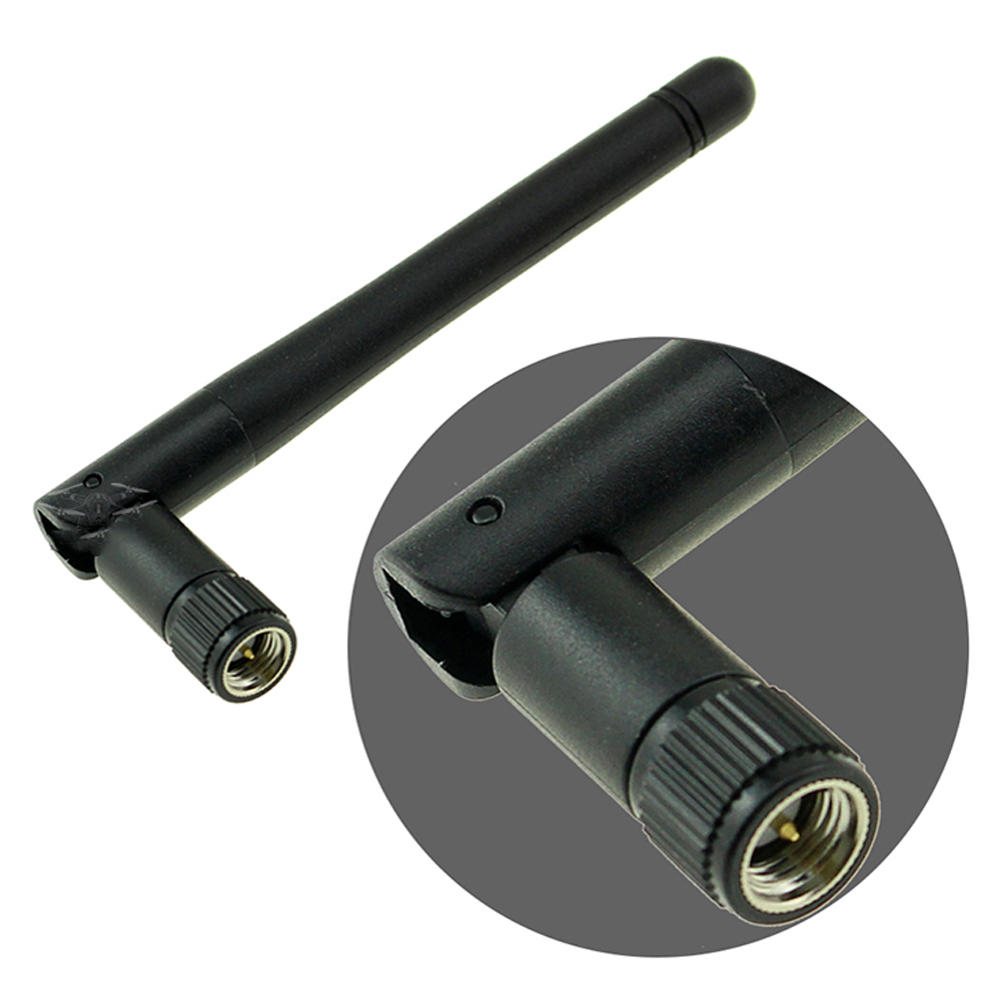
\includegraphics[width=3in]{telemmodule.jpg}

\caption{916MHz telemetry module \cite{telemModule}.}

\label{mavStruct}
\end{figure}

\subsection{Results and Discussion}
This section of the paper will be about the overall set up of the system, the design process, and the problems that were encountered on the way.
\subsubsection{System Set Up}
Our data transmission system starts in the Pixhawk scheduler code within the main file called ArduPlane.cpp. The flight controller is essentially a microcontroller without an operating system, which means that it needs to implement a scheduling system that figures out which process out of hundreds for the processor to run. The scheduler code can be found in figure ~\ref{mavSched}.
% MAX PICTURE 3
\begin{figure}[h!]
\hspace*{0cm}
\centering
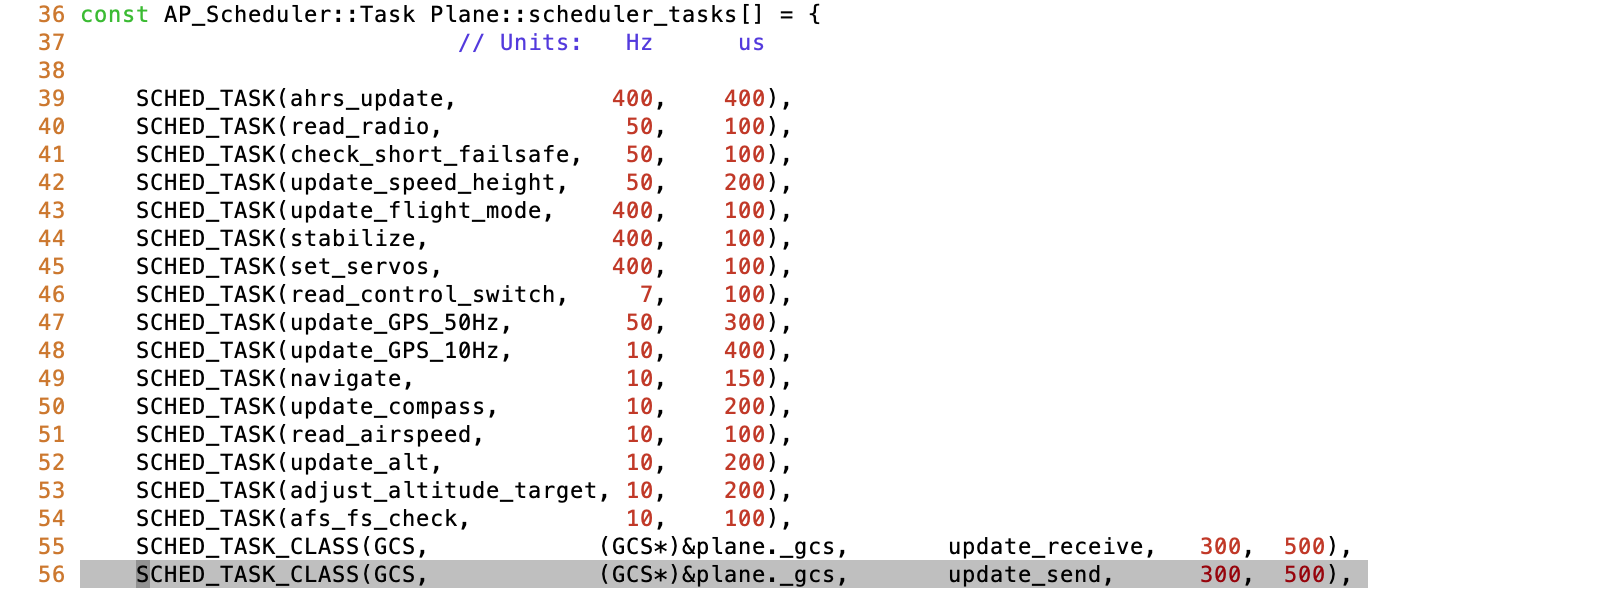
\includegraphics[width=3in]{Scheduler.png}
\caption{Ardupilot scheduler}
\label{mavSched}
\end{figure}

The highlighted line of code in figure ~\ref{mavSched} schedules the GCS sending module, which calls functions to use the MAVLink link between the ground station and the plane. Diving deeper into the code base in the plane folder, there is the GCS\_MAVLink.cpp file that contains the functions to actually go about sending the message. This code can be found in figure ~\ref{gcsMav}.

% MAX PICTURE 4
\begin{figure}[h!]
\hspace*{0cm}
\centering
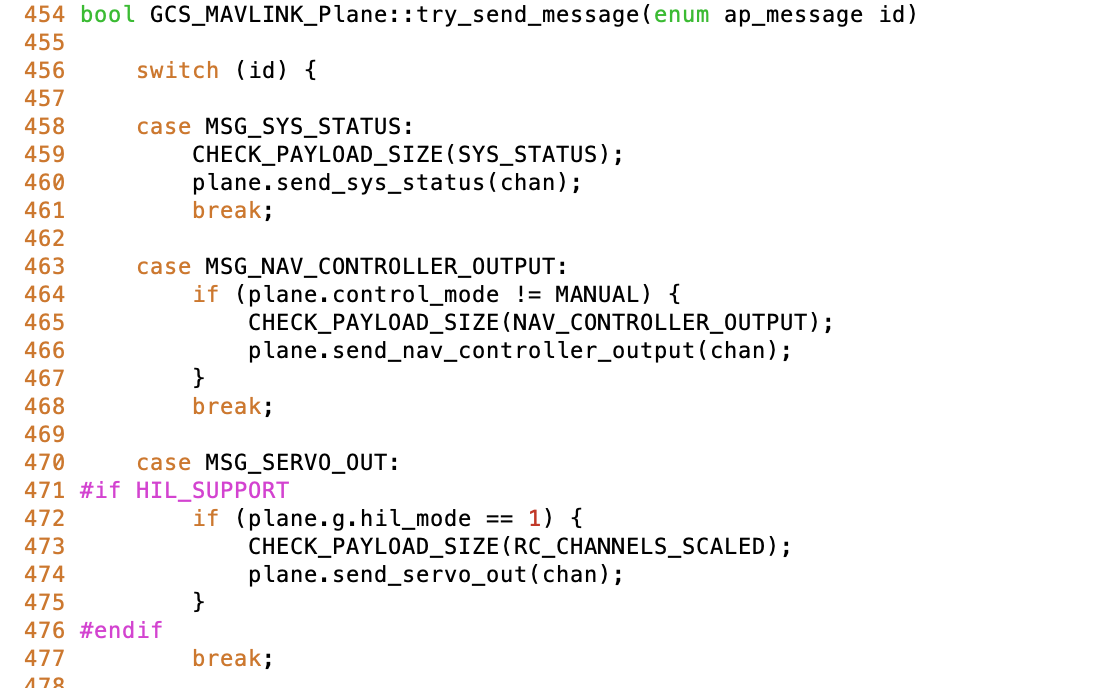
\includegraphics[width=3in]{GCS_Mavlink.png}
\caption{Vehicle specific MAVLink sending function}
\label{gcsMav}
\end{figure}

As a backup to the function in figure ~\ref{mavSched}, ArduPilot also implemented a function that all vehicles under the ArduPilot umbrella use. If none of the IDs passed into the try\_send\_message function matched, it would fall into the try\_send\_message that was defined in the libraries of ArduPilot. This was good for the overall project structuring, but made figuring out the actual implementation of MAVLink transmission very challenging. 

Figure ~\ref{fallthrough} is the fallback function at the end of the try\_send\_message function that links the plane MAVLink implementation to the common MAVLink packets that all ArduPilot vehicles use. This function is contained in the library files that all ArduPilot vehicles have access to. 
% MAX PICTURE 5
\begin{figure}[h!]
\hspace*{0cm}
\centering
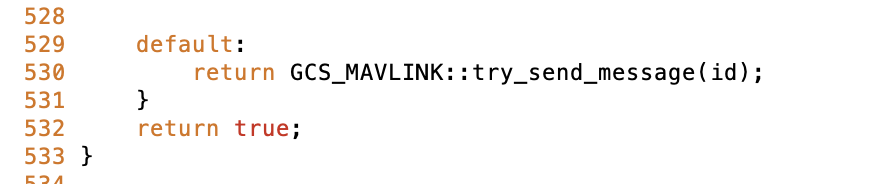
\includegraphics[width=3in]{Fallthrough.png}
\caption{Sending function common to all Ardupilot vehicles}
\label{fallthrough}
\end{figure}

By editing code in either the library try\_send\_message function or the ArduPlane specific try\_send\_message function, I as able to make changes to the MAVLink messages that were being sent to the ground station. 
I changed existing MAVLink definitions rather than create new ones because of the difficulty in changing the MAVLink protocol version from version 1.0 to version 2.0 (please view the problems section for more information on this issue). I started by selecting messages to overwrite in the common.xml file. An example of the XML code can be found in figure ~\ref{xml}.


\begin{figure}[h!]
\hspace*{0cm}
\centering
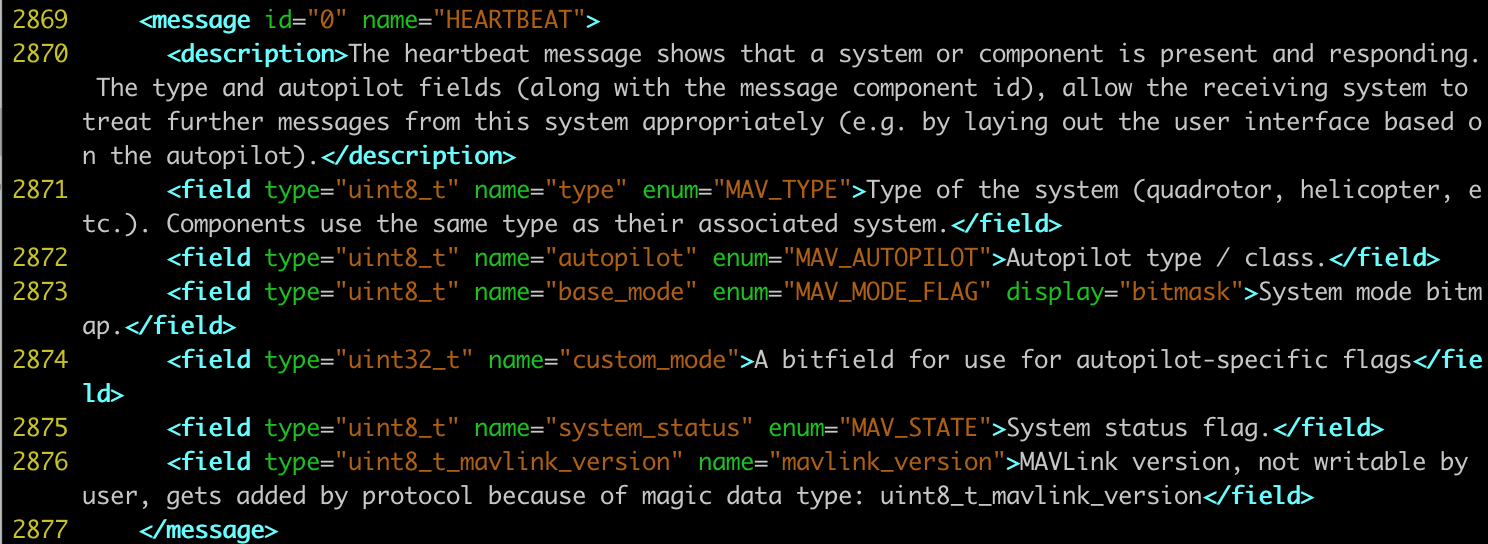
\includegraphics[width=3in]{message.png}
\caption{XML definitions of MAVLink packets}
\label{xml}
\end{figure}

\subsubsection{Design Process}
I began the design process by trying to prevent the flight controller from having to handle any of the data transmission at all. Instead, my original plan was to have a Teensy microcontroller serve as the gateway between the ground station on the ground and the plane up in the sky. The first thing that I did was to set up a UART link between the Teensy and the flight controller, sending over information that would eventually be relayed to the ground station. The overall structure can be found in figure ~\ref{version1}.
% MAX PICTURE 6
\begin{figure}[h!]
\hspace*{0cm}
\centering
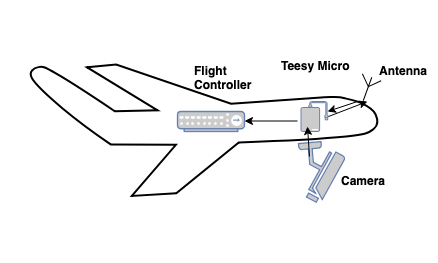
\includegraphics[width=3.5in]{Version1.png}
\caption{Diagram of dual microcontroller setup}
\label{version1}
\end{figure}

However, this original set up became less than optimal when the incredible wealth of the already existing ground control software became apparent. I discovered that the ground control software, Mission Planner, could be used to send GPS waypoints to the plane which the plane would then track to without any extra code. The interface between the flight controller and the ground control station would only work if it could receive bytes from the ground station. This required the flight controller to have a direct link to the ground station which it was not configured to do in the first design. 

It didn't make sense to spend a lot of time designing a system where the Teensy acted as a go-between for the flight controller and ground station. In addition, the small and underpowered Teesny with a processor clocked at 48 MHz could not hope to keep up with a flight controller clocked at over 3 times that. The Teensy was then removed from the picture, letting the flight controller bear a greater computational load. A diagram of the second design can be found in figure ~\ref{version2}.

% MAX PICTURE 7
\begin{figure}[h!]
\hspace*{0cm}
\centering
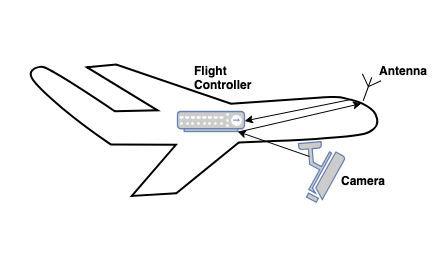
\includegraphics[width=3in]{Version2.png}
\caption{Updated design without Teensy microcontroller}
\label{version2}
\end{figure}

While this new set up removed complexity from the system, it placed a lot more stress on the flight controller. Instead of just flying the plane and keeping the control systems in check, it had to do image processing work for the IR camera. To reduce the stress on the flight controller, we decided to place the Teensy micro back on board. It would be in charge of performing all fire detection. The flight controller would listen on a serial port for a signal from the Teensy for whether a fire was detected. The flight controller's only added load would then only be to send out one extra MAVLink packet and listen on a serial port. This is far less stressful than trying to squeeze image processing into an already tightly scheduled system. The final design layout can be found in figure ~\ref{version3}.

% MAX PICTURE 8
\begin{figure}[h!]
\hspace*{0cm}
\centering
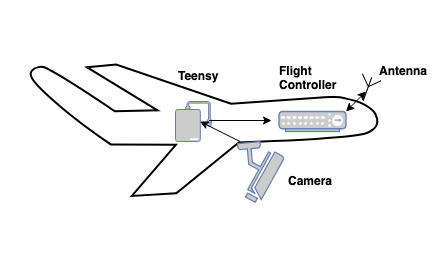
\includegraphics[width=3in]{Version3.png}
\caption{Final design}
\label{version3}
\end{figure}

After the two computing devices had their roles clearly set, the design process began anew. The first important thing to do was to get a good understanding all of the underlying code for data transmission in the ArduPilot framework. After tracking down the control flow through the different files which eventually ended in in the library file that all ArduPilot vehicles used, the next step was to add a particular message to the common.xml file which contained the MAVLink message definitions. 

Due to a parameter problem that I will cover in-depth in the problems part of this discussion, I found it necessary to overwrite one of the existing MAVLink definitions. The HIL\_STATE message with ID 90 was selected because it had been replaced by another message and was no longer in use. This message was overwritten with a custom packet that contained fire detection data. This packet would only be sent when the sensing apparatus detected a fire. The simple control flow of this setup can be found in figure ~\ref{sending}.

% MAX PICTURE 9
\begin{figure}[h!]
\hspace*{0cm}
\centering
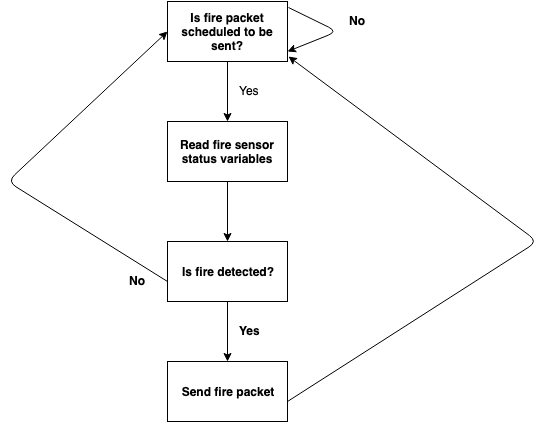
\includegraphics[width=3in]{Sending.png}
\caption{Control flow of fire packet transmission algorithm}
\label{sending}
\end{figure}

I wrote a Python script on the ground station side that used the Python package PyMavlink. This script read the serial port incoming messages would enter on and translate the incoming data into a human readable form. The associated data was then used to make plots, such as the one in figure ~\ref{flyingGraph} that plots latitude and longitude from the incoming GPS data packets.

This allows for the collection of real time flight data which can be very different from the data read from a wind tunnel in the lab. 

% MAX PICTURE 10
\begin{figure}[h!]
\hspace*{0cm}
\centering
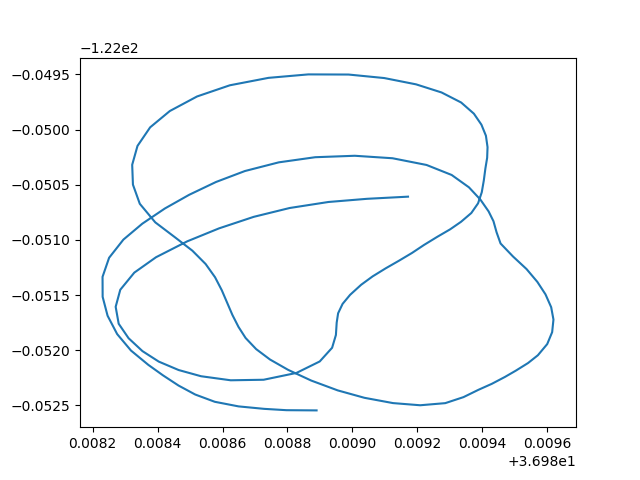
\includegraphics[width=3.5in]{flight02-22-2019_maiden.png}
\caption{Plot of the aircraft's maiden flight using GPS coordinates that were logged in real time via the telemetry link.}
\label{flyingGraph}
\end{figure}

\subsubsection{Design Problems}
The biggest and most enveloping design problem I encountered during this project was changing the MAVLink protocol version. Please note the MAVLink byte structure referred to in the next few sentences is the first diagram of data transmission section of the report. The 5th byte of the packet designates the ID number that corresponds to the MAVLink message. This limits the total number of incoming messages to 256. The common.xml file contains message definitions up to 256. Due to the limited number of bits (8) that correspond to the incoming ID, there are only 256 possible messages that can be sent. This is why overwriting the already defined messages in the common.xml file is needed. Creating new messages with an ID value greater than 255 could not be sent by the current MAVLink protocol.

I realized this when I created a custom packet with an ID value of 11065 and tried to send it. However, nothing was sent, not even garbage. This along with the packet header of 0xFE made it very clear that the first version of the MAVLink protocol was used rather than the updated and more flexible MAVLink version 2. Overwriting the message was a necessary evil to send custom packets. 

The changing of this protocol is badly documented on the ArduPilot website. Eventually, a manual change using the MAVProxy Python library was attempted (specifically changing the protocol version parameter of MAVLink), but MAVLink 1 packets continued to be sent. In the interest of time, I decided that simply overwriting the useless packets defined for MAVLink 1 was the best course of action.

An added problem of working with this flight controller is the time and processing constraints that adding a custom bit of functionality to an already extremely overtasked system come with. However, by keeping subroutines short, it was possible to add a good amount of data collecting and transmission software to an already built system.

\subsection{Data Transfer Conclusion}
Data transmission software is essential to pulling real time data that closely reflects and explains the events that occurred during flight. Even though the open source autopilot is incredibly difficult to parse through and overall not very well written by industry computer science standards, it can be manipulated to add custom MAVLink functionality. Once the difficultly of working with different transmission protocols over several different programming languages is overcome, data transfer's extreme value can be truly realized. 

% Kodiak
\section{Control System}
\subsection{Introduction}
The control systems section will explore the art of controlling planes without a pilot on-board. The overall plan is to control the aircraft in an optimal way to detect wildfires, but we are just focused on control in general for now.

\subsubsection{Treating the Aircraft as a Dubins Vehicle}
This section focuses on creating a model for guidance and path following. Using coordinate frame matrices to resemble flight, we can model aircraft dynamics along with outside forces with the following equation (eq 9.9 in \cite{S-U-A}):
\[ \begin{pmatrix}
\dot{p_n} \\
\dot{p_e} \\
\dot{h}
\end{pmatrix} 
= V_a \begin{pmatrix}
cos(\psi) \\
sin(\psi) \\
0
\end{pmatrix}
+ \begin{pmatrix}
w_n \\
w_e \\
0
\end{pmatrix}
\]
It essentially says that the angular roll rate $\dot{p}$, and the rate of change in altitude $\dot{h}$ are equivalent to the airspeed $V_a$ times the cosine and sine of the yaw angle $\psi$ plus the wind direction $w$. Note that aerodynamic forces acting on the aircraft body are removed from this equation to greatly simplify it. The equation assumes the aircraft maintains a steady altitude to model it like a Dubins vehicle with a forward velocity and a turning rate. The airplane is then controlled by increasing or decreasing the velocity and changing the turning rate. Below in Figure \ref{f8} is a plot of a Dubins vehicle moving in a figure-eight pattern:
\begin{figure}[h!]
\hspace*{0cm}
\centering
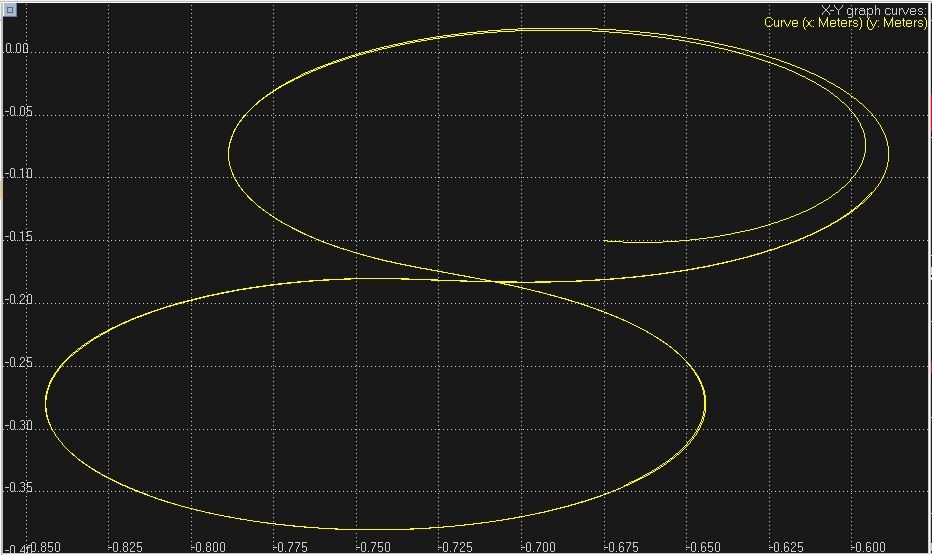
\includegraphics[width=3in]{dubins_fig8.jpg}
\caption{Dubins vehicle programmed to move in a figure-eight pattern by holding a constant velocity and changing the sign of its turning rate at a specific time interval. An airplane at a constant forward velocity and altitude can be modeled in a similar fashion. Note this picture was taken from a project the author, Kodiak, completed for CMPE 141.}
\label{f8}
\end{figure}
This idea is particularly useful for Unmanned Aerial Vehicles (UAVs), which do not perform aerobatic maneuvers and usually maintain a steady altitude to scan an area. Engineers can basically pretend their UAV is a Dubins vehicle once it reaches its cruising altitude! We can then relate the rotation rate along the vertical axis $\dot{\psi}$ to gravity, velocity, and the roll angle $\phi$ with the following equation (eq 9.14 in \cite{S-U-A}):
\[ \dot{\psi} = \frac{g}{V_a}tan(\phi) \]
It is important because it gives us a direct relation from roll angle to turning rate. This equation is similar to the steering wheel on a car - it rolls left and right to make the car turn left and right. In this case, the aircraft itself is the steering wheel rolling left and right to change its heading. We now have everything we need to control a UAV like a Dubins vehicle using the roll angle to modify turning rate, and the motor to adjust its speed.

\subsubsection{Aircraft Ground Control Stations}
A ground control station is something that can apply the Dubins vehicle model as the UAV is in the air. As an operator plans the flight, the ground control software will calculate the turning rate (i.e. roll angle) required to follow the path. If the turning rate is unachievable, the software must notify the operator, or perform longer, wider maneuvers to correct for the error and follow the path as close as possible. This is one of many reasons why ground station are important tools for a UAVs. Their other purposes are to allow an operator to track/plan the mission, observe flight status, and pilot the aircraft. ``Depending upon range and type of mission (complexity of the UAV system), smaller UAVs are controlled via visual contact (manual real-time control), while the larger ones are equipped with a communication system (engage stored on-board flight plans)" (\cite{U-A-D}, p. 141). Some UAVs are not fully autonomous, so an operator must fly it using a laptop with ground control software. UAVs also have various sensors on them like a weapon position sensor, altimeter, airspeed sensor, inertial measurement unit (IMU), and many more. If the ground control station operator notices anything is working improperly, he can take full control and act accordingly.
\begin{figure}[h!]
\hspace*{0cm}
\centering
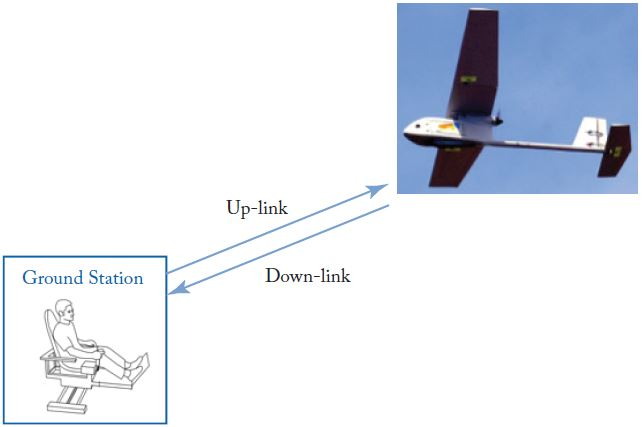
\includegraphics[width=3in]{groundControl.jpg}
\caption{Diagram displaying and operator of a ground control station to pilot an aircraft. Most stations do not require the operator to sit in a cockpit-like seat, but the exaggeration is useful for a novice UAV enthusiast. \cite{U-A-D}, p. 142, Figure 8.1.}
\label{gcDiagram}
\end{figure}
Normally, there are two operators to a ground control station; the vehicle flight operator and the mission payload operator. The flight operator is in charge of keeping the machine in the air, while the payload operator interfaces with other aircraft systems. This could be aiming and firing guns, taking weather data, or gathering recon information for teams on the ground. These operators play a crucial role because although the plane can fly mostly, or fully autonomously, ``most UAV losses are attributed to operator errors" (\cite{U-A-D}, p. 143). The operators must be comfortable when working with these expensive devices or else their state of mind will fatigue, and the chances of making a mistake increase. It is important to keep comfort in mind when designing a ground control station.

\subsubsection{Glider Soaring via Reinforcement Learning in the Field \cite{GliderBirds}}
One way to extend the flight time of a small, unmanned aircraft is to utilize thermals and updrafts similar to the way birds do. Physicists at UC San Diego figured out how to do exactly that by using reinforcement learning - a type of machine learning.
\begin{figure}[h!]
\hspace*{0cm}
\centering
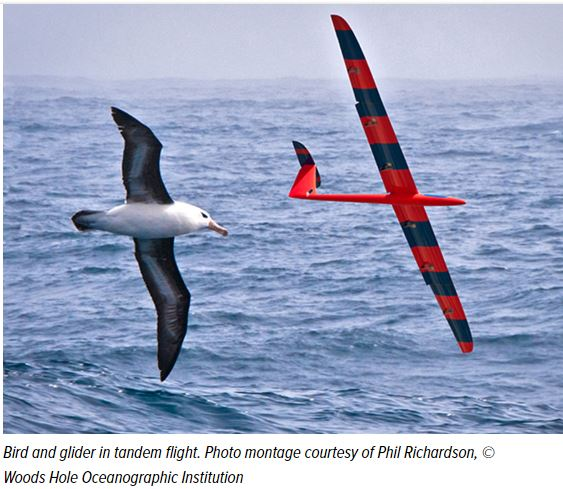
\includegraphics[width=3in]{gliderAndBird.jpg}
\caption{Here is one of the gliders used in the testing process flying in tandem with a seagull. The two both have the same attitude because they are tracking thermals or updrafts in a similar manner. \cite{gbArticle}}
\label{gliderAndBird}
\end{figure}
Reinforcement learning is essentially a way for a system to learn based on trial and error; if it preforms an action and things go well, it remembers that as a good choice, while on the other hand, poor situations from bad maneuvers are kept in the ``don't do again" list. The physicists started by simulating gliders in turbulent wind flow to find important parameters that improve navigation through a thermal. They then moved on to testing a real plane with a 2 meter wingspan. The plane was equipped with a flight controller running modified ArduPlane code to pilot the aircraft through updrafts. Researchers soon discovered that they needed to write algorithms to estimate ``environmental cues" to maneuver the glider in such a way to gain the most lift out of the environment. For example, when a pocket of greater lift is at a diagonal to the aircraft's forward heading, banking in a proper manner will generate more lift. This project intends to apply these properties to the Forever Flight aircraft to achieve a longer flight time when searching for wildfires.

\subsection{Methods}
\subsubsection{Choice of Aircraft Frame}
For our UAV, the team decided to go with a glider style aircraft over a delta-wing style. We originally wanted to use a delta-wing because they are quick to build and durable. However, we learned that these characteristics should not be our main focus because they define what someone would want if they were planning on a lot! Since we were creating a plane intended to fly forever, we realized that we should choose an efficient-flying plane that can use less power to remain in the air. We wanted a plane that can utilize updrafts or thermals to recharge its battery when running low, or to simply gain altitude free of charge. Therefore, a glider was an obvious choice. The team built a cardboard glider but did not have much luck flying it; the aircraft had unstable pitch oscillations despite the center of gravity being perfect. It ended up crashing, but served as a good tool to learn how to connect all of the electronics. (see Figure \ref{pitchOsc}). Fortunately around that time, we received funding and were able to purchase a well designed plane. It has a 2.6m wingspan to generate a ton of lift, and it has an optimal amount of area for solar cell placement. This new plane has no pitch oscillations and flies very well.
\begin{figure}[h!]
\hspace*{0cm}
\centering
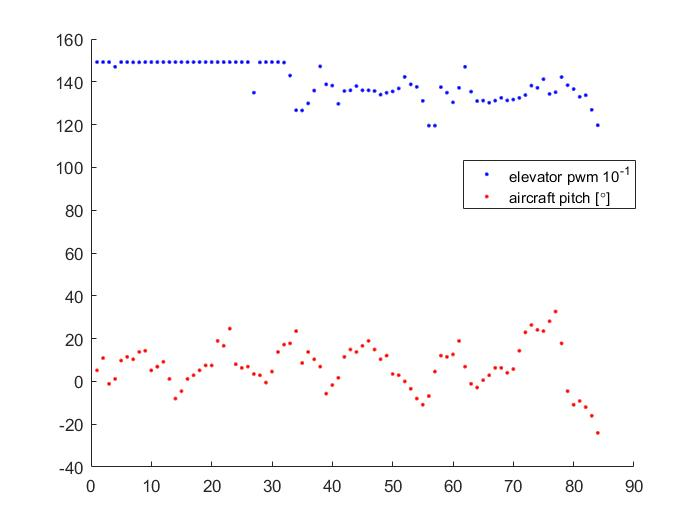
\includegraphics[width=3in]{pitch_elevPWM.jpg}
\caption{This plot if of aircraft pitch (red) and elevator deflection (blue) in PWM over the flight duration. A decrease in elevator PWM equates to the control surface deflecting upward, i.e. it causes the aircraft to pitch up. Notice that only pitch up elevator was applied throughout the entire flight, however the plane pitched up and down. This made it clear that the plane was not flying properly. Rather than spending time debugging the issue, we purchased a new plane that was guaranteed to fly well.}
\label{gliderAndBird}
\end{figure}
\subsubsection{Tasks to Connect the Electronics}
The first step in connecting the control system is to verify that all electronics are working properly before inserting them into the plane. This involves testing the servos and motor in a simple RC configuration without any autopilot, then connecting them to the autopilot and ensuring manual control can be taken with the flip of a switch, and finally integrating the wireless data transmission system.
\subsubsection{Simple RC Configuration}
Before motors and servos can be tested, the Taranis X9D RC transmitter must be bound to the FrSky X8R receiver so the two can communicate.
\begin{enumerate}
\item With the X9D off, hold down the F/S button on the receiver and power it up. Then let go of the F/S button. The light on the receiver should be solid RED indicating it is in bind mode.
\item Turn the X9D on and select the model you want to bind the receiver to.
\item Short press the menu button, and then press the page button to navigate to page 2 of the settings.
\item Scroll down with the `+' or `-' buttons until you see ``Channel Range" and ``Receiver No." settings.
\item Under ``Receiver No.", highlight [bind] and press ``ENT" to confirm. Leave the ``Channel Range" as 1-8 with telemetry ON. Press ``ENT" again.
\item The receiver's LED will flash GREEN and RED, and the transmitter will beep, indicating that they are binding.
\item After a couple beeps, press ``EXIT" on the transmitter and power off the receiver.
\item Power the receiver back on. The LED should turn solid GREEN after a few seconds indicating that it is connected to the transmitter. The two are now paired together under the selected model forever unless the receiver is re-bound to a different model.
\end{enumerate}

With that done, servos and motors can be controlled by plugging them into the outputs on the X8R. Power everything off and plug the ESC and four servos into the receiver (see Table \ref{x8rChannels}). Note that the two aileron servos are connected to only one channel using a servo Y-splitter. This causes the servos to behave opposite of one another as they would on a typical aircraft. The motor connects to the ESC via three wires with bullet connectors (see Figure \ref{motorToEsc}).
\begin{table}[h!]
\caption{FrSky X8R Channels to Aircraft Control Surfaces}
\centering
\begin{tabular}{|c|c|}
\hline
X8R Channel & Aircraft Control Surface \\
\hline
1 & Ailerons \\
\hline
2 & Elevator \\
\hline
3 & Motor \\
\hline
4 & Rudder\\
\hline
\end{tabular}
\label{x8rChannels}
\end{table}

\begin{figure}[h!]
\hspace*{0cm}
\centering
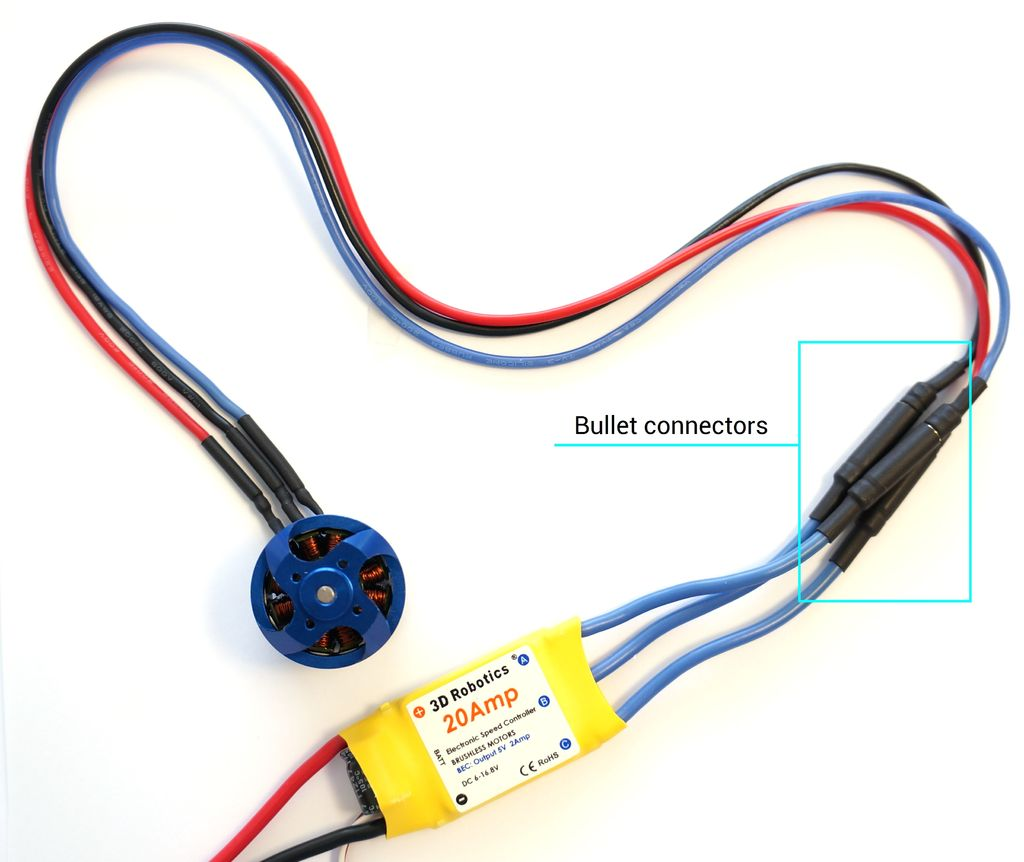
\includegraphics[width=3in]{motorToEsc.jpg}
\caption{Brushless motor connected to ESC via bullet connectors found it \cite{mToE}}
\label{motorToEsc}
\end{figure}
Now that everything is connected, follow these steps to center servos and test servo/motor functionality.

\begin{enumerate}
\item Ensure the propellers is OFF of the motor shaft, and the transmitter is powered off.
\item Turn on the transmitter.
\begin{enumerate}
\item Ensure all switches are in default position and throttle position is at its minimum (default settings on the X9D will cause it to yell at you if these constraints are not met).
\end{enumerate}
\item Plug the battery into the ESC.
\begin{enumerate}
\item The servos will center right when they receive power for the first time. Make sure that the trim on all channels is centered.
\end{enumerate}
\item Wait for the motor startup sound sequence to play.
\item Move sticks on the transmitter and observe control behavior.
\begin{enumerate}
\item Note that servo direction can be flipped in the transmitter settings, so their directions are not too important at this point.
\item If the motor spins in the wrong direction when the throttle is applied, switch any two of the three wires that connect it to the ESC.
\end{enumerate}
\end{enumerate}

In this stage, it is also wise to manually calibrate the ESC so it recognizes this specific transmitter's maximum and minimum PWM throttle outputs. Follow the steps below.

\begin{enumerate}
\item Ensure the propellers is OFF of the motor shaft, and the transmitter is powered off.
\item Place the throttle stick to its maximum position.
\item Plug the battery into the ESC.
\begin{enumerate}
\item It will play a special sequence to indicate that maximum throttle has been detected.
\end{enumerate}
\item Place the throttle stick to its minimum position within 2 seconds.
\begin{enumerate}
\item The ESC will beep and play its normal startup sequence.
\item If the normal startup sequence does not play and instead the ESC beeps abnormally, repeat this process and be sure to move the throttle stick to the minimum position within 2 seconds!
\end{enumerate}
\item Calibration is now complete.
\end{enumerate}

With these steps complete, we can move to connecting the motors, servos, and receiver to the flight controller.

\subsubsection{Connect Motors, Servos, and Receiver to Pixhawk}
Refer to Figure \ref{mainScheme} for the wiring diagram of all the electronics connected to the flight controller. Note that a special cable is required to connect the signal port of the LiPo Cell Voltage Monitor to the TELEM1 port on the Pixhawk. This can be purchased from Craft and Theory, or one can be made using an RS232 converter. We decided to buy the \$15 connector. Also observe that although not intuitive, the Pixhawk's IO PWM Out is connected to the PMB's FMU PWM In. This is to map the RC outputs to the FMU header pins rather than to the M1-8 solder pads. This is not described very well in the Pixhawk's quickstart guide!

With all components connected, the first step is to run through Mission Planner's setup wizard. This involves calibrating sensors on the Pixhawk, flashing it with the latest firmware, choosing the battery sensor module, and configuring the Taranis X9D so Mission Planner recognizes its PWM outputs. If incorrect PWM values are observed, or they do not change with stick movements, navigate to ``Initial Setup" $\rightarrow$ ``Servo Output". Then change each channel function from throttle, ailerons, elevator, and rudder to their respective RCINx channels as defined in Table \ref{x8rChannels}.

The next step is to configure the flight modes in mission planner so switches on the X9D can cycle through different modes. If the preconfigured Flight Deck model is used (described in the next section), RC channel 5 will be mapped to switches SD and SC. Play with these to set the preferred flight mode selections. With everything powered on, when one of those switches is flicked, one can see the flight mode change from gray to green in Mission Planner. Now when in MANUAL or STABILIZE mode, and the flight controller armed (1 second press on the GPS safety switch), the X9D should have full control of the motor and servos!\\

\begin{figure*}[h]
\hspace*{0cm}
\centering
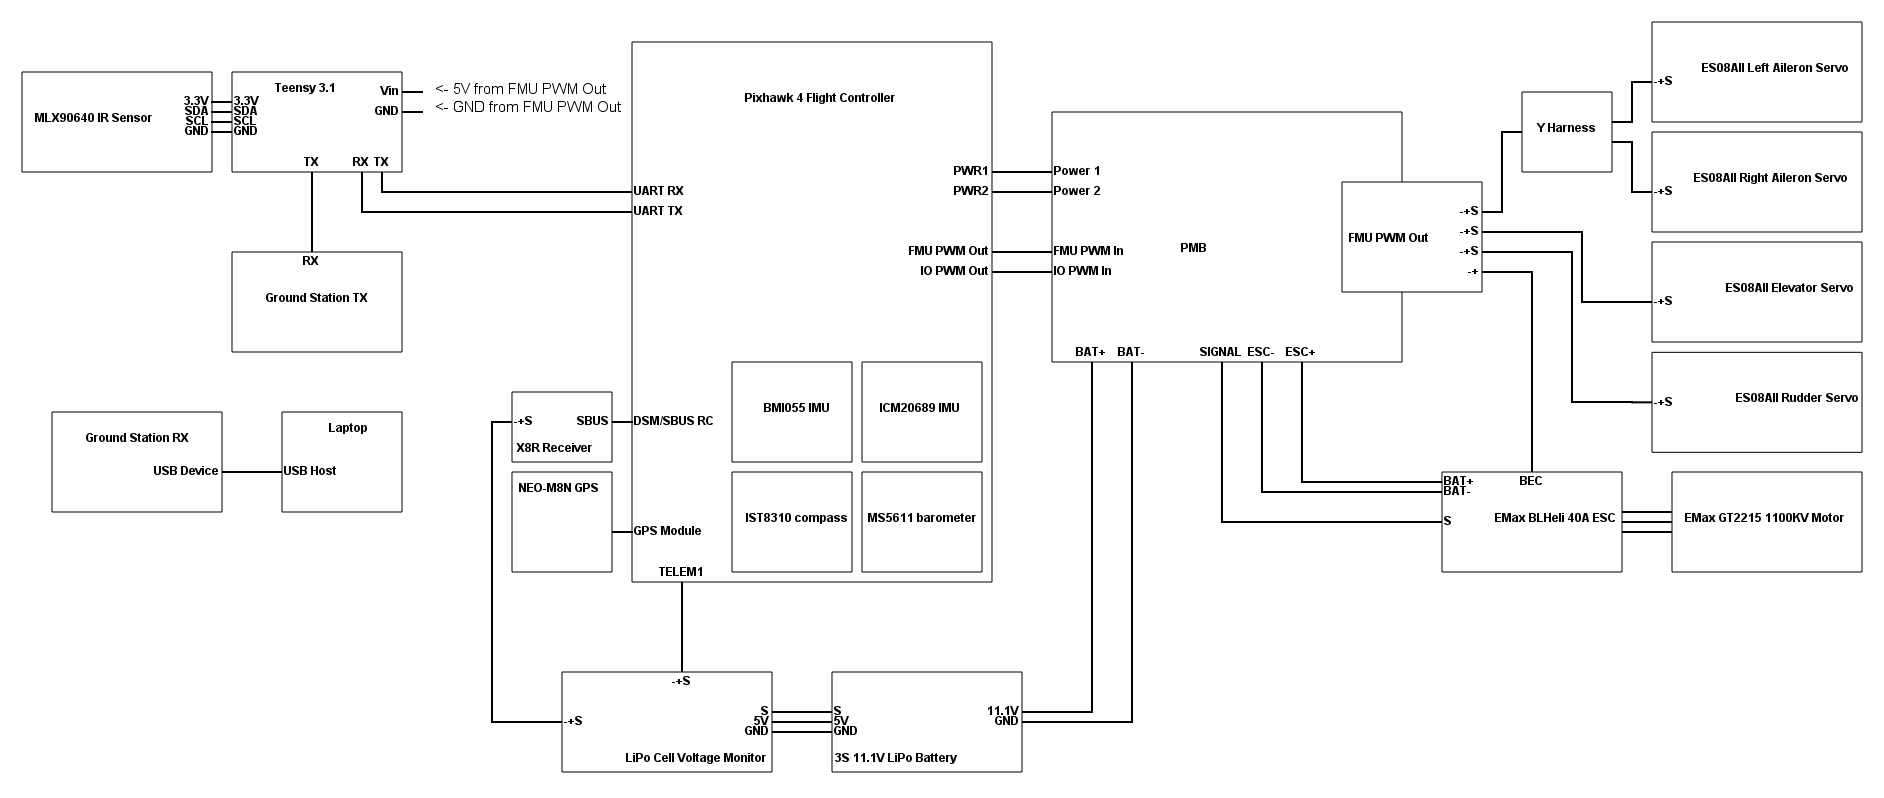
\includegraphics[width=\textwidth]{hardwareBlockDiagram.png}
\caption{Diagram of all electronics in the aircraft.}
\label{mainScheme}
\end{figure*}

\subsubsection{Flash Taranis X9D with FlightDeck Software}
The FlighDeck software from Craft and Theory can serve as a backup ground station directly on the transmitter. It provides everything necessary to fly the aircraft such as heading, altitude, battery voltage, and attitude. Follow the steps below to flash FlighDeck onto the transmitter after purchasing it from Craft and Theory. Note that a 40\% discount is given on FlightDeck when it is purchased together with the TELEM cable described in the section above.
\begin{enumerate}
\item Download OpenTx Companion at\\ \href{https://www.open-tx.org}{https://www.open-tx.org}.
\begin{enumerate}
\item Run the companion executable.
\item Select radio type `FrSky Taranis X9D+' (or a different radio that is being used).
\item Check the `lua' box and ensure the `sql5font' box is unchecked.
\end{enumerate}
\item Download latest firmware version.
\begin{enumerate}
\item We used this one:\\ \href{https://www.open-tx.org/2019/01/06/opentx-2.2.3}{https://www.open-tx.org/2019/01/06/opentx-2.2.3}.
\end{enumerate}
\item Put Taranis in bootloader mode by holding both horizontal trims inward and powering on.
\item Connect Taranis to computer with mini-USB cable.
\item Flash firmware to radio using OpenTx Companion's handy user interface.
\item Navigate to SD card drive on the computer that the Taranis is plugged into. It is drive E:\textbackslash on my laptop. It contains folder such ad LOGS, MODELS, and SOUNDS.
\item Copy all of these files and back them up in a safe location.
\item Download the latest SD card version at\\ \href{https://downloads.open-tx.org/2.2/sdcard/opentx-x9d%2B/}{https://downloads.open-tx.org/2.2/sdcard/opentx-x9d\%2B/}. % note the first % does not make a comment
\item Extract the contents of the .zip folder into the root directory of the SD card (in my case, drive E:\textbackslash).
\item Download FlightDeck.zip from the email confirmation when it was bought or from the Craft and Theory account created for the purchase.
\item Extract the contents of the ``SDcard" folder directly into the root directory of the Taranis SD card (in my case, drive E:\textbackslash).
\begin{enumerate}
\item Make sure to merge the contents of these folders and replace/overwrite any file already on the SD card.
\end{enumerate}
\item Manually backup all models currently on the X9D to its SD card before proceeding to avoid any potential frustration.
\begin{enumerate}
\item Long press `Enter' over each model and select `Backup'.
\end{enumerate}
\item Add the preconfigured FlightDeck model to the transmitter using OpenTx Companion.
\begin{enumerate}
\item Open the X9D+.otx file that came with FlightDeck in OpenTx Companion.
\item Press the ``Write Models and Settings to Radio" button.
\end{enumerate}
\item Unplug the USB cable from the Taranis, select `Exit', and confirm. The radio will now boot up normally.
\item Discover new sensors!
\begin{enumerate}
\item In Mission Planner, navigate to the full parameter list and set ``SERIAL1" = 10 for FrSky SPORT Passthrough, OpenTx.
\item Disconnect from Mission Planner and unplug the micro USB cable.
\item Power the electronics with a battery and wait for the Pixhawk startup sequence to play.
\item Navigate to the Telemetry screen on the X9D and select the ``discover new sensors" button.
\item Notice that GPS and CELS (battery lowest cell voltage), amongst others are now available.
\end{enumerate}
\end{enumerate}

\subsection{Mounting the Electronics in the Plane}
Now with the electronics tried and tested, it is time for the moment we have all been waiting for - to stuff everything inside of the plane. When doing this, it is important to mount the flight controller and GPS as close to the aircraft's center of gravity as possible. It is also important to keep other data transmission antennas (like the GPS and Telemetry link antennas) far away from another to reduce noise generated between the two. Keep the plane's center of gravity in mind when finding a nice place for heavier equipment. It must balance on two points 1/4 of the distance of the chord behind the leading edge of the wing, and preferably be slightly nose heavy. Failure to do this will cause the plane to fly improperly and will likely ensue a crash.

After mounting everything, power up the transmitter, connect the battery to the flight controller and test that all control surfaces move in the correct direction based on manual stick input. Then verify that the plane balances properly over its center of gravity. If it does not, shift something heavy (the battery works well) to correct this. Once all of these checks pass, the plane is ready for manual flight!

\section{Fire Detection System}

\subsection{Introduction}
The fire detection system onboard the aircraft scans a stream of images for signs of fire. These images are captured by an Infrared camera. A background on the inner workings of this camera will be given below. Infrared imaging is only one of many feasible techniques. An overview of other techniques explored by other researchers will also be given. Finally, this section will detail the fire detection system implementation, the advantages of our implementation, and the drawbacks of our implementation. 

\subsection{Comparison of Techniques} \label{fire_comparison_section}
\subsubsection{Human Observation}
There are many tried and true methods for detecting wildfires. The oldest, and most simple method is to station human beings in watch towers in high elevation positions, such as the ridge lines of mountains. This method is not prone to false positives, as human beings are very good at identifying a fire once they see it. Human beings can detect fire through many senses, such as visible smoke, visible flames, burning smells, and changes in temperature or humidity. However, human vision has a limited range. A large number of watch towers and human watchers are necessary to monitor a small area. Also, the logistics of watch towers are complex. New watch towers take time to construct, the system is not mobile. The system also places human beings in danger. A fire could easily spread after detection but before being extinguished, and burn down the watch tower. 

\subsubsection{Manned Aerial Observation}
A more recent technique uses human observers inside large manned aircraft. Unlike the watch tower method, this system keeps human beings out of harms way. This system also has the advantage of being mobile, as a plane can be deployed anywhere. The range of this method is also less limited, as a plane cover an area much larger than a human's vision in a single flight. Large enough planes can even be equipped to combat fires when they are detected. 

The downsides of manned aircraft are cost and complexity. Flying a plane is an expensive activity. It also takes a highly trained pilot, and a team of people to maintain the vehicle. The fire department of a small rural town will lack the resources to use this method. Instead, they must rely on the state to provide the aircraft, pilot, and maintenance crew. Unfortunately, small rural towns are most affected by wildfires. 

\subsubsection{Satellite Imagery}
Satellite imagery is another technique employed to detect wildfires. Satellites have an enormous upfront cost, but thankfully many space agencies allow small organizations to access their imagery. Many spaces agencies also allow organizations to place custom modules onboard their satellites, in the form of "Cube Satellites". However, the major drawback of using satellites to detect fires lies in the technical details. Satellite imagery has a very slow frame rate, on the order of days \cite{technique_review}. This delay is simply not suitable. In the span of a day, a fire can grow to an enormous size. With the right combination of weather and fuel, a wildfire can grow at a rate of 300 feet per second \cite{climate_and_wildfire}.

Satellite imagery has another crucial downside: low resolution. Satellites orbit at very high altitudes, on the order of hundreds and thousands of miles above earth's surface \cite{technique_review}. Advanced camera equipment would not be able to detect small fires. Satellite imagery would likely only capture large scale artifacts of fire, like smoke trails. However, these only develop after a fire has grown to a considerable size. If the goal of fire detection is to catch fires early, then satellites are not the right tool for the job. 

\subsubsection{Optical Camera Imagery}
Many real world fire detection systems employ optical cameras. These operate in much the same way as a human observer, and are positioned in high elevation positions. They look horizontally over a region, and the resulting images can be digitally processed, or manually monitored for signs of smoke and fire. A major downside of this approach is the horizontal camera orientation. In densely forested areas, a fire may be obscured by trees while it is small. Optical imagery also cannot be used at night, as smoke is nearly impossible to distinguish in the dark. 

The figure below demonstrates an optical image processing algorithm produced by Cruz et al. \cite{ffdi}. For each pixel of an input image, the algorithm computes the probability that the pixel is part of a fire. 

\begin{figure}[H]
\centering
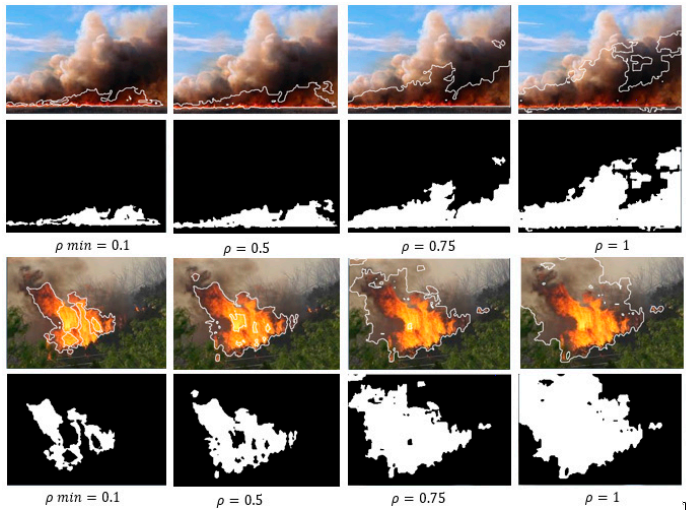
\includegraphics[width=3.5in]{ffdi.png}
\caption{The Forest Fire Detection Index algorithm with $\rho$ values of 0.1, 0.5, 0.75, 1, and 1.25. 
Note that the region considered as being "on fire" grows in size with larger values of $\rho$. For values above 0.75, the 
algorithm mistakenly classifies smoke as part of the fire. }
\label{ffdi_image}
\end{figure}

\subsection{Infrared Sensor Background}
An infrared sensor is a specific type of spectrometer, which is a device capable of converting electromagnetic radiation into an electrical signal. Spectrometers can be tuned to be sensitive to different wavelengths of radiation. An infrared sensor is tuned to produce the maximum response signal when it receives radiation in the Infrared Region. 

According to Planck's Law, all matter radiates energy in proportion to its temperature. The hotter an object is, the more energy it radiates. Plank's Law also tells us that the wavelength at which the most energy is produced decreases with temperature. In other words, hotter objects radiate higher frequency energy, and more total energy than colder objects. The figure below shows various Planck curves, which relate energy, temperature, and wavelength.

\begin{figure}[h]
\centering
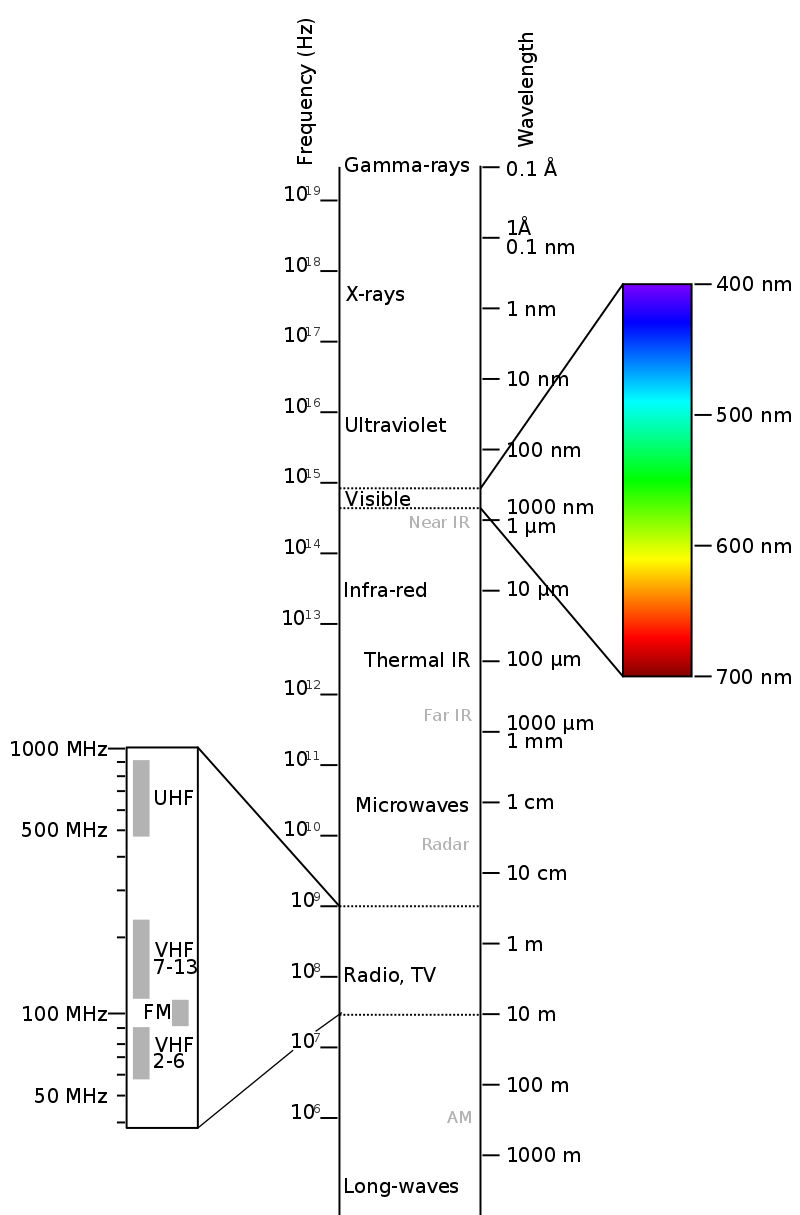
\includegraphics[width=3.5in]{em_spectrum.png}
\caption{The electromagnetic spectrum. Radiation between wavelengths of 1$\mu$m and 1000$\mu$m is classified as Infrared Radiation}
\label{em_spectrum_image}
\end{figure}

There are several wavelength bands within the Infrared Region. The Thermal Infrared Region occupies wavelengths of 8-15 $\mu$m. 
The Medium Wave Infrared Region occupies wavelengths of 3-5$\mu$m. A peak in the Thermal Infrared Region range indicates an object that is roughly 248K. 
The Thermal Infrared Region is not appropriate for our application, because wood burns at 573-973K \cite{estimating_wildfire}.
Instead, we will use the Medium Wave Infrared Region. 
A peak in this region indicates an object that is between 600K and 900K.

\begin{figure}[h]
\centering
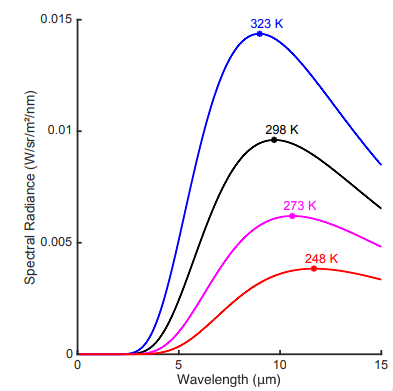
\includegraphics[width=3.5in]{plancka.png}
\caption{Planck curves for temperatures 323K, 298K, 273K, and 248K. Notice that as temperature decreases, the peak wavelength increases and the total area under the curve decreases. This means that the temperature of an object can be detected, if we know the peak wavelength of its electromagnetic radiation.}
\label{plancka_image}
\end{figure}

\begin{figure}[h]
\centering
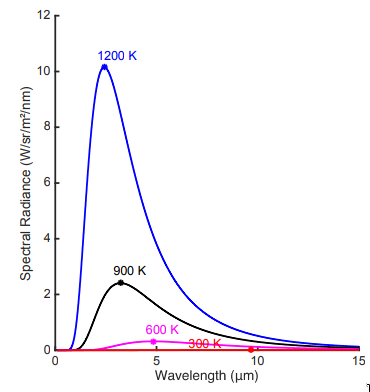
\includegraphics[width=3.5in]{planckb.png}
\caption{Planck curves for temperatures 1200K, 900K, 600K, and 300K}
\label{planckb_image}
\end{figure}

\subsubsection{Infrared Imagery}
Infrared imagery uses a grid of infrared sensors to create an image. Each sensor corresponds to a single pixel, and 
varies its electrical resistance in response to infrared radiation that collides with the sensor's surface. Infrared imagery has a 
key advantage over optical imagery, because IR radiation can be detected in night or day, and can detect objects that are merely hot, and not actually on fire. IR radiation is also not obstructed by smoke or fog, which could obscure the sight line of an
optical imagery fire detection system.

\subsection{Fire Detection System Implementation}
Our fire detection system makes use of an MLX90640, which is a low cost infrared sensor array. The MLX90640
produces images with a resolution of 32 horizontal pixels and 24 vertical pixels. The lens on the camera 
gives it a 55 degree horizontal field of view, and a 35 degree vertical field of view. The figure below
shows the pyramid that encloses the sensor's field of view. 

\begin{figure}[h]
\centering

\includegraphics[width=3.5in]{mlx90640_fov.png}
\caption{From a height of 400 feet, images captured by the MLX90640 have a physical width of 416 feet and height of 252 feet.
Each pixel represents a 13x10 square foot region.}
\end{figure}

Each pixel represents a 13x10 square foot region, which is the smallest detectable fire size. Any fire smaller than this 
will not register on the camera, and therefore cannot be detected by the system.

Image \ref{fire_detection_algorithm} describes the algorithm that backs the fire detection system. 

\begin{figure}[h]
\centering

\includegraphics[width=3.5in]{fire_detection_algorithm.png}
\caption{Fire detection algorithm}
\label{fire_detection_algorithm}
\end{figure} 

Upon receiving a fire size message, the main microcontroller transmits
the current GPS location, current time, and fire size value to the ground station.

\subsection{Limitations and Problems}
The minimum detectable fire size is a crucial metric of our system. The smaller it is, the smaller the fire will be when first responders arrive. The smaller it is, the easier it is to suppress the fire. This metric depends on the cruising altitude of the aircraft, and the resolution of the camera. This system was only tested at heights below 400 feet, due to FAA regulations. In practice, the cruising altitude should be higher, to mitigate collision with trees or terrain. This negatively affects the minimum detectable fire size. This can be compensated for with a higher resolution camera, however thermal cameras rapidly increase in price with increasing resolution. In short, using higher resolution thermal cameras is not a scalable solution. Using regular optical cameras is one solution, but these have many drawbacks, as discussed in section \ref{fire_comparison_section}. 
Our fire detection system produces relatively simple information. It records its current GPS location and the current time whenever it flies over a fire. However, there are many more characteristics about a fire that are relevant to fire fighters. 

Fire fighters are interested in modeling fires. The location of the starting point of a fire is nice to know, but it is equally important to know what the fire will do after it has started. Fire models attempt to describe the intensity, forward rate of spread, perimeter growth rate, area of perimeter, and shape of perimeter. 

Intensity is defined as energy released per unit time, per unit length of the fire’s perimeter. For example, a fire burning in a forest will typically have a higher intensity than a fire in a grassland. This is because the available fuel is much denser in a forest than in grasslands.

The forward rate of spread of a fire is the speed at which a particular point on the perimeter of the fire advances. This metric has units of distance per unit time. For example, the recent Paradise fire reached a forward rate of spread of 100 yards per second. The forward rate of spread is large when a fire moves uphill, and is positively affected by wind speeds.

The rate of spread, or rate of perimeter growth is self descriptive. It also has units of distance per unit time. An extremely large fire could have a small forward rate of spread, but a large rate of perimeter growth.

These models depend on information about the fire, such as location, the moisture content of the fuel, the wind speed, the wind direction, and the slope of the surrounding terrain. Figure \ref{fire_shape}, produced by F. Albini \cite{estimating_wildfire}, shows different shapes of fire, depending on wind speed.

\begin{figure}[h!]
\hspace*{0cm}
\centering
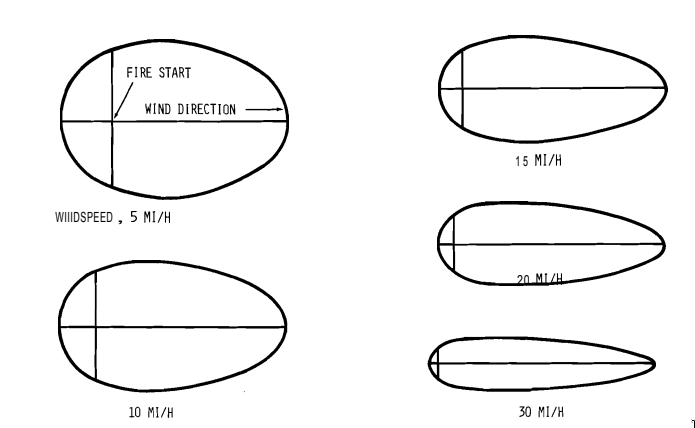
\includegraphics[width=3.5in]{fire_shape.png}
\caption{Approximate fire shapes (not sizes, the scales are arbitrary) for windspeeds of 5, 10, 15, 20, and 30 mi/h \cite{estimating_wildfire}}
\label{fire_shape}
\end{figure}

It is important to keep in mind that models are only an approximation of true fire behavior, and are inherently inaccurate. Fires are also difficult and dangerous to reproduce in a laboratory setting. A large, realistic wildfire would never be purposely started for the sake of measurement. This means that data on wildfires is hard to come by, and of low quality. A model may also be inaccurate if certain assumptions are broken. Many models assume that the region on fire is composed of a single fuel source, which is uniformly dense.

\subsection{Future Work}
Given these additional fire characteristics, it is only natural that our project's scope should expand and provide additional information, beyond the location of a fire's starting point. Image recognition techniques could be used to measure the area of land covered by a fire. Similarly, image recognition could be used to describe the shape of a fire. This information is useful to fire fighters, because it allows them to predict the rate of spread, and the direction of travel of a fire. It will likely take first responders a non-trivial amount of time to arrive at the scene of a fire, and this information gives them some idea of what to expect. A fire will grow in the meantime between detection and fire fighter response. 

\section{Conclusion}
We now have a control system implemented and ready to be simulated. We do not want to immediately jump into autonomous mode because if it does not work as we expect, the plane might crash, or fly far away and never return. For this reason, we are designing a Software in the Loop (SITL) simulation to detect any bugs in the autonomous code. One has been found already where if the aircraft is launched in the opposite direction from its first GPS waypoint, it will never turn around! The ArduPlane code tries to fly the plane around the entire world to hit the waypoint, but since our plane does not have enough battery life to make the journey, it would crash. Future work includes more simulation, and testing the autopilot in real time once we feel we have found all the bugs and we know how to avoid them.

\appendices
\section*{Appendix}

\section*{Acknowledgements}
Kodiak would like to thank the authors of Small Unmanned Aircraft, and Unmanned Aircraft Design for providing such detailed descriptions on UAV design and control. He would also like to thank all researchers that are apart of Glider soaring via reinforcement learning in the field \cite{GliderBirds} for conducting such excellent work that will contribute to his capstone project.

Max would like to thank Precision Hawk for giving us around two thousand dollars of electronic equipment for free. We would also like to thank the people on forums online that provided help describing ArduPilot functionality.

\begin{thebibliography}{2}
% Max's citations
\bibitem{Ardupilot source}
``ArduPlane Home," ArduPilot. [Online]. Available: http://ardupilot.org/plane/index.html. [Accessed: 06-Mar-2019].
\bibitem{MAVLink packet structure}
``MAVLink," Wikipedia, 08-Nov-2018. [Online]. Available: https://en.wikipedia.org/wiki/MAVLink\#Packet\_Structure. [Accessed: 05-Mar-2019].
\bibitem{Pixhawk basics}
``Pixhawk 4," Basic Concepts · PX4 User Guide. [Online]. Available: https://docs.px4.io/en/flight\_controller/pixhawk4.html. [Accessed: 06-Mar-2019].
\bibitem{Teensy info}
``Teensy v3.1 - 32 bit arduino-compatible microcontroller board," Velleman Spotlight. [Online]. Available: 
https://www.velleman.eu/products/view\linebreak?id=420178\&country=be\&lang=en. [Accessed: 06-Mar-2019].

\bibitem{telemModule}


``Banggood.com, “3DR Radio Telemetry Kit With Case 433MHZ 915MHZ For MWC APM PX4 Pixhawk for FPV RC Airplane RC Toys \& Hobbies from Toys Hobbies and Robot on banggood.com,” www.banggood.com. [Online]. Available: https://bit.ly/2JisfKa [Accessed: 18-Mar-2019].


% Kodiak's citations
\bibitem{S-U-A}
Beard, R. and McLain, T. (2012). Small unmanned aircraft. Princeton, N.J: Princeton University Press.

\bibitem{gbArticle}
C. Dillon, "Physicists Train Robotic Gliders to Soar like Birds", Ucsdnews.ucsd.edu, 2018. [Online]. Available: https://ucsdnews.ucsd.edu/pressrelease/physicists-train-robotic-gliders-to-soar-like-birds. [Accessed: 20-Feb-2019].

\bibitem{GliderBirds}
G. Reddy, J. Wong-Ng, A. Celani, T. Sejnowski and M. Vergassola, "Glider soaring via reinforcement learning in the field", Nature, vol. 562, no. 7726, 2018. Available: 10.1038/s41586-018-0533-0.

\bibitem{mToE}
``Motor to ESC," Instructables. [Online]. Available: https://www.instructables.com/id/Beginners-Guide-to-Connecting-Your-RC-Plane-Electr/ [Accessed: 07-March-2018].

\bibitem{U-A-D}
Sadraey, M. (n.d.). Unmanned aircraft design.

% Zane's citations
\bibitem{electromagnetic_spectrum}
"Electromagnetic spectrum", en.wikipedia.org, 2019. [Online]. Available: https://en.wikipedia.org/wiki/Electromagnetic\_spectrum. [Accessed: 18- Mar- 2019].

\bibitem{ffdi}
H. Cruz, M. Eckert, J. Meneses and J. Martinez, Efficient Forest Fire Detection Index for Application in Unmanned Aerial Systems (UASs). Madrid: Research Center on Software Technologies and Multimedia Systems for Sustainability (CITSEM), 2016.

\bibitem{technique_review}
A. Alkhatib, A Review on Forest Fire Detection Techniques. Hindawi Publishing Corporation, 2014.

\bibitem{leaf_crops}
C. Chen, Determining the Leaf Emissivity of Three Crops by Infrared Thermometry. Taichung: MDPI Sensors, 2015.

\bibitem{airborne_optical}
R. Allison, J. Johnston, G. Craig and S. Jennings, Airborne Optical and Thermal Remote Sensing for Wildfire Detection and Monitoring. MDPI Sensors, 2016.

\bibitem{estimating_wildfire}
USDA Forest Service, "Estimating Wildfire Behavior and Effects", United States Department of Agriculture, Ogden, Utah, 1976.

\bibitem{wireless_sensors}
D. Doolin and N. Sitar, Wireless sensors for wildfire monitoring. Berkeley: University of California, Berkeley, 2005.

\bibitem{climate_and_wildfire}
[7]A. Westerling, A. Gershunov, T. Brown, D. Cayan and M. Dettinger, Climate and Wildfire in the Western United States. San Diego: American Meteorological Society, 2003.

\bibitem{multisensor_network}
I. Bosch, A. Serrano and L. Vergara, Multisensor Network System for Wildfire Detection Using Infrared Image Processing. Valencia, Spain: Hindawi Publishing Corporation, 2013.
\end{thebibliography}

\vspace{1cm}

% Kodiak's amazing bio
\textbf{Kodiak North}
is currently a senior at the University of California - Santa Cruz. He is majoring in Robotics Engineering, and looking for a career in the new drone industry once he graduates. On his free time, Kodiak enjoys surfing, repairing his truck, and flying his RC race quadcopter.

\textbf{Maxwell Bradley}
is a senior at UC Santa Cruz. He is a computer engineering major specializing in computer system, which dabbles in both hardware and software. He will be continuing into the computer engineering MS program here at UCSC after he completes his bachelors, and hopes to work for himself after he graduates. When he isn't laboring over some piece of code, he enjoys distance running, playing the guitar, and checking out breweries.

% Zane's bio
\textbf{Zane Bradley}
is a 4th year Computer Engineering student at the University of California, Santa Cruz. He loves to hiking, traveling, listening to music, and programming in his free time.




% insert where needed to balance the two columns on the last page with
% biographies
%\newpage

%\begin{IEEEbiographynophoto}{Jane Doe}
%Biography text here.
%\end{IEEEbiographynophoto}

% You can push biographies down or up by placing
% a \vfill before or after them. The appropriate
% use of \vfill depends on what kind of text is
% on the last page and whether or not the columns
% are being equalized.

%\vfill

% Can be used to pull up biographies so that the bottom of the last one
% is flush with the other column.
%\enlargethispage{-5in}

\end{document}

